\providecommand{\main}{../..}
\documentclass[\main/notes.tex]{subfiles}

\begin{document}
	\setcounter{chapter}{10}
	\chapter{Systems Analysis}
		\section{An Overview of Systems Development}
			\begin{definition}{The Development Team}
				A team that consists of users, managers, systems development specialists, various support personnel and other stakeholders.

				Responsible for determining the objectives of the new information system, and delivering a system that meets these objectives.

				\begin{description}
					\item[Project] A planned collection of activities that achieves a goal, such as constructing a new manufacturing plant, or developing a new decision support system. Should have as defined starting and ending point.
					\item[Project Manager] A manager that is responsible for coordinating all people and resources needed to complete the project on time. Can be an IS person inside the organisation, or an external consultant. They need technical, business, and people skills. Usually responsible for controlling project quality, training personnel, facilitating communication, managing risks, and acquiring any necessary equipment.
					\item[Stakeholders] People who, either themselves or through the area of the organisation they represent, ultimately benefit from the systems development project.
					\item[Users] People who will interact with the system regularly. Can be employees, managers, or suppliers.
					\item[Systems Analyst] A professional who specialises in analysing and designing business systems.
						\begin{description}
							\item[Specialist Business Analysts] Experts in the business who try to identify ways in which new information systems can improve the current business processes.
						\end{description}
					\item[Programmer] Responsible for modifying or developing programs to satisfy user requirements. A programmer  takes plans from the systems analyst, and builds or modifies the necessary software.
					\item[Team Leader] Responsible for the development team. Can be from the IS department, a manager from the company, or a consultant. Needs both technical and people skills.
				\end{description}
			\end{definition}
			\subsection[Information Systems Planning]{Information Systems Planning and Aligning Organisation and IS Goals}
				\begin{definition}{Information Systems Planning}
					Translating strategic and organisational goals into systems development initiatives.

					Strategic goals must be finite, measurable, and tangible.
				\end{definition}
				\begin{sidenote}{The Steps of IS Planning}
					\begin{center}
						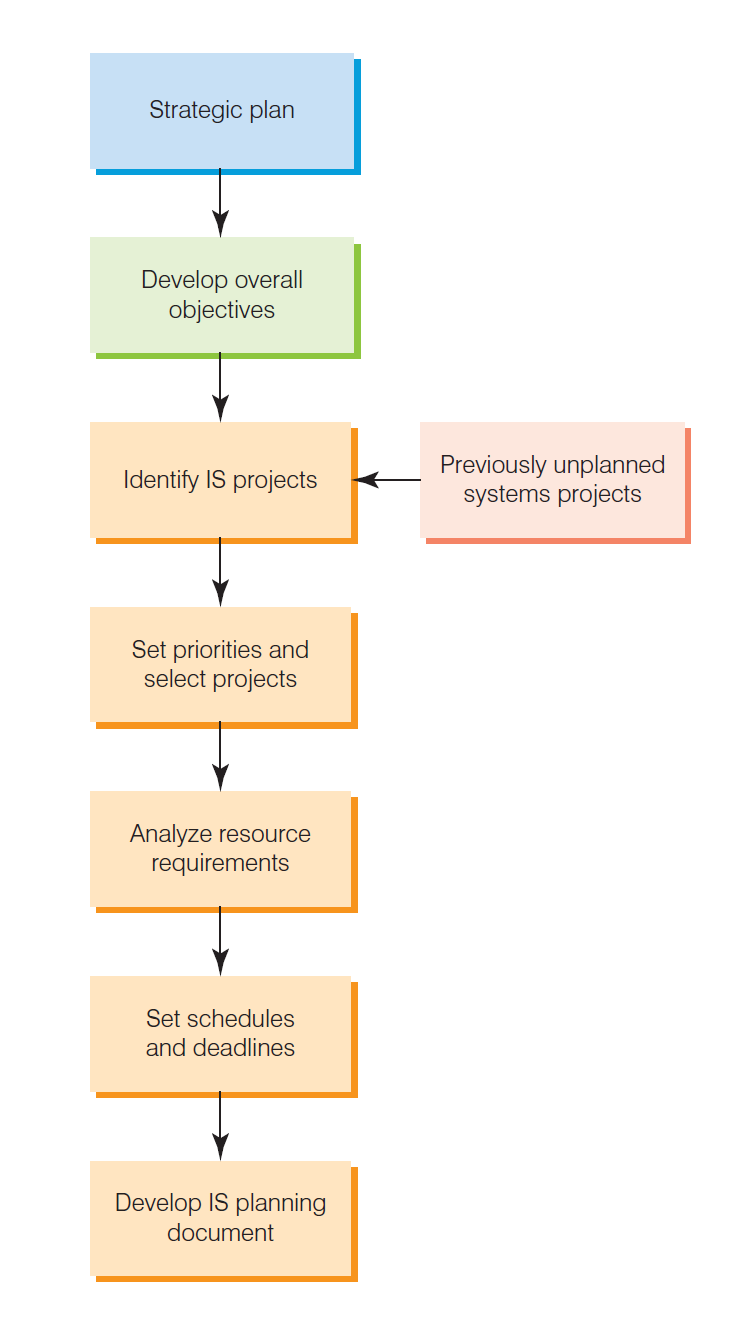
\includegraphics[width=0.6\textwidth]{chapter11/is_planning_steps.png}
					\end{center}
				\end{sidenote}
				\pagebreak
				\begin{definition}{Creative Analysis}
					The investigation of new approaches to existing problems. 

					Typically, inspired by people and events not directly related to the problem.
				\end{definition}
				\begin{definition}{Critical Analysis}
					The unbiased and careful questioning of whether system elements are related in the most effective ways.
					\begin{itemize}[nosep]
						\item Question statements and assumptions.
						\item Identify and resolve objectives and orientations that conflict.
					\end{itemize}
				\end{definition}
			\subsection{Establishing Objectives for Systems Development}
				\begin{sidenote}{Overall Objective}
					The overall objective of systems development is to achieve business goals, not technical goals, by delivering the right information to the right person at the right time.
				\end{sidenote}
				\begin{definition}{Critical Success Factors (CSFs)}
					Factors that are essential to the success of certain function areas of an organisation.
				\end{definition}
				\begin{definition}{Performance Objectives}
					The extent to which a system performs as desired.
					\begin{multicols}{2}
						\begin{itemize}[nosep]
							\item The quality or usefulness of the output
							\item The accuracy of the output
							\item The quality or usefulness of the format of the output
							\item The speed at which output is generated
							\item The scalability of the resulting system
							\item The degree to which business risk is reduced
						\end{itemize}
					\end{multicols}
				\end{definition}
				\begin{definition}{Cost Objectives}
					The costs associated with the system, should be minimised.
					\begin{multicols}{2}
						\begin{itemize}[nosep]
							\item Development costs
							\item Costs related to the uniqueness of the system application
							\item Fixed investments in hardware and related equipment
							\item Ongoing operating costs of the system
						\end{itemize}
					\end{multicols}
				\end{definition}
				Performance objectives and cost objectives should be balanced.

		\pagebreak
		\section{Systems Development Lifecycles (SDLC)}
			The systems development process is also called the \concept{systems development lifecycle (SDLC)}.
			\subsection{The Traditional Systems Development Lifecycle}
				\begin{definition}{Traditional Systems Development Lifecycle}
					Also known as the \concept{waterfall approach}.

					\begin{minipage}[t]{0.44\textwidth}
						\vspace{0pt}
						\begin{center}
							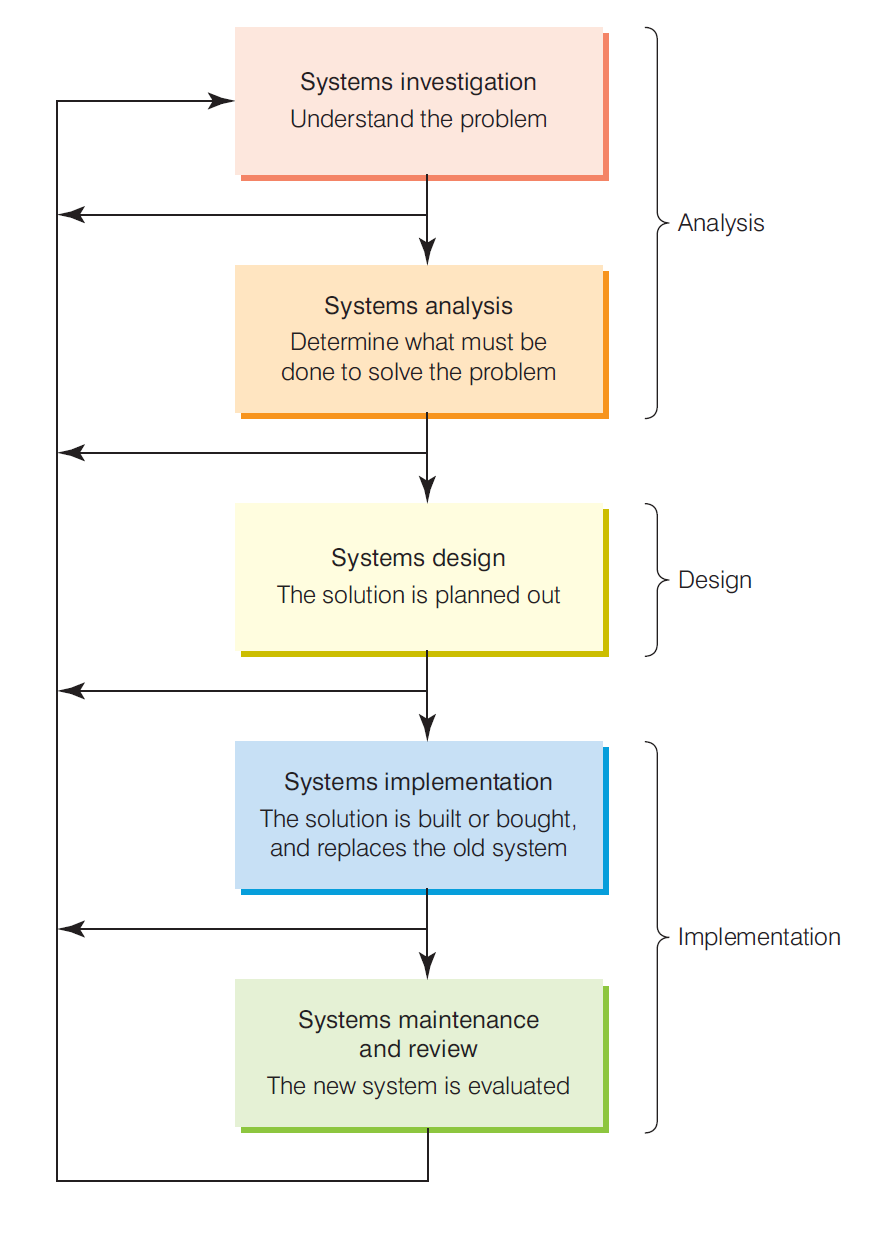
\includegraphics[width=0.95\linewidth]{chapter11/traditional_sdlc.png}
						\end{center}
					\end{minipage}
					\begin{minipage}[t]{0.55\textwidth}
						\vspace{0pt}
						\begin{description}
							\item[Systems Investigation] Problems and opportunities are identified and considered in light of the goals of the business. The result of this phase is a defined development project.
							\item[Systems Analysis] `What must the IS do to solve the problem?' Studies existing systems and work processes to identify strengths, weaknesses, and opportunities for improvement. The result of this phase is a list of requirements and priorities.
							\item[Systems Design] `How will the IS do what it must do to obtain the problem solution?' The result of this phase is a technical design that either describes the new system, or describes how existing systems will be modified.
							\item[Systems Implementation] Creating or buying the various system components detailed in the system design. The result of this phase is an installed, operational information system that meets the business needs for which it was developed.
							\item[Systems Maintenance and Review] Ensure that the system operates as intended, and modify the system so that it continues to meet changing business needs.
						\end{description}
					\end{minipage}
					\begin{center}
						\begin{tblr}{colspec={>{\raggedright}X|>{\raggedright}X}, row{1}={font=\bfseries}, row{even}={white}}
							Advantages & Disadvantages\\
							\midrule
							Formal review at the end of each phase allows maximum management control. & Users get a system that meets the needs as understood by the developers.\\
							Creates considerable system documentation. & Documentation expensive and time-consuming, and difficult to keep current.\\
							Formal docs ensure system requirements can be traced back to business needs. & User needs are unstated or misunderstood.\\
							Produces reviewable intermediate products. & Not easy for user to review intermediate products.
						\end{tblr}
					\end{center}
				\end{definition}
			\subsection{Prototyping}
				\begin{definition}{Prototyping}
					Also known as the \concept{evolutionary lifecycle}. Takes an iterative approach to systems development. During each iteration, requirements and alternative solutions to the problem are identified and analysed, new solutions are designed, and a portion of the system is implemented.
					\begin{description}
						\item[Operational Prototype] A prototype that has functionality -- it does something towards solving the problem. May accept input, partially process it, and output the results.
						\item[Non-operational Prototype] A mock-up or model. Includes input specifications and formats. Can be developed much faster than an operational prototype.
					\end{description}
					\begin{center}
						\begin{tblr}{colspec={>{\raggedright}X|>{\raggedright}X}, row{1}={font=\bfseries}, row{even}={white}}
							Advantages & Disadvantages\\
							\midrule
							Users can try the system and provide constructive feedback during development. & The final solution might be only incrementally better than the initial solution.\\
							An operational prototype can be produced in weeks & Formal end-of-phase reviews might not occur. It is difficult to contain the scope of the prototype -- the project never seems to end.\\
							As solutions emerge, users become more positive about the process and the results & System documentation is often absent or incomplete.\\
							Enables early detection of errors and omissions. & System backup and recovery, performance, and security issues can be overlooked in the haste to develop a prototype.
						\end{tblr}
					\end{center}
				\end{definition}
			\subsection{Other Systems Development Approaches}
				\begin{definition}{Rapid Application Development (RAD)}
					A systems development approach that employs tools, techniques, and methodologies designed to speed application development.

					Reduces paper-based documentation, automatically generates program source code, and facilitates user participation in design and development activities.
					\begin{description}
						\item[Joint Application Development (JAD)] Used for data collection and requirements analysis. Involves group meetings in which users, stakeholders, and IS professionals work together to analyse existing systems, propose possible solutions, and define the requirements for a new or modified system. Often uses \concept{group support systems (GSS)} software to foster positive group interactions.
					\end{description}
					Generally, RAD is better suited for DSS's and MIS's, and less well suited for TPS's.
				\end{definition}
				\pagebreak
				\begin{sidenote}{Advantages and Disadvantages of RAD}
					\begin{center}
						\begin{tblr}{colspec={>{\raggedright}X|>{\raggedright}X}, row{1}={font=\bfseries}, row{even}={white}}
							Advantages & Disadvantages\\
							\midrule
							Puts an application into production sooner than any other approach & Can burn out systems developers and other project participants\\
							Documentation is produced as a by-product of completing project tasks & Requires systems analysts and users to be skilled in RAD systems development tools and RAD techniques.\\
							Forces teamwork and lots of interaction between users and stakeholders & Requires a larger percentage of stakeholders' and users' time than other approaches.
						\end{tblr}
					\end{center}
				\end{sidenote}
				\begin{definition}{Agile Development}
					Allows the systems to change as they are being developed. Requires frequent face-to-face meetings with the systems developers and users as they modify, refine, and test how the system meets users' needs, and what its capabilities are.
					\begin{description}
						\item[Extreme Programming (XP)] Uses pairs of programmers who work together to design, test, and code parts of the systems they develop.
					\end{description}
				\end{definition}
			\subsection{The End-User Systems Development Lifecycle}
				\begin{definition}{End-User Systems Development Lifecycle}
					Any systems development project in which business managers and users assume the primary effort.
				\end{definition}
			\subsection{Outsourcing and On-Demand Computing}
				\begin{sidenote}{Outsourcing}
					A good idea if:
					\begin{itemize}[nosep]
						\item A company believes it can cut costs.
						\item A firm has limited opportunity to distinguish itself competitively through a particular IS operation or application.
						\item Uninterrupted IS service is not crucial.
						\item Outsourcing does not strip the company of technical know-how required for future IS innovation.
						\item The firm's existing IS capabilities are limited, ineffective, or technically inferior.
						\item A firm is downsizing.
							\begin{description}
								\item[Downsizing] Reducing the number of employees or managers, equipment and systems, and even functions and departments. 
							\end{description}
					\end{itemize}
				\end{sidenote}
			\subsection{Genetic Programming}
				\begin{definition}{Genetic Programming}
					An approach to creating computer code based on natural selection. Initially random code evolves through numerous iterations to become a program that solves a set problem.
				\end{definition}

		\section{Factors Affecting System Development Success}
			\begin{sidenote}{Factors Affecting System Development Success}
				\begin{itemize}[nosep]
					\item Involvement
					\item Degree of Change
					\item The ability to manage change
					\item Quality of project planning, and standards
				\end{itemize}
			\end{sidenote}
			\begin{sidenote}{Project Planning Issues}
				\begin{center}
					\begin{tblr}{colspec={>{\raggedright}X>{\raggedright}X}, row{1}={font=\bfseries}, row{even}={white}}
						Factor & Countermeasure\\
						\midrule
						Solving the wrong problem. & Establish a clear connection between the project and organisational goals.\\
						Poor problem definition and analysis & Follow a standard systems development approach.\\
						Poor communication & No easy solution.\\
						Project is too ambitious & Narrow the project focus to address only the most important business opportunities.\\
						Lack of top management support. & Identify the senior manager who has the most to gain from the success of the project, and recruit this person to champion the project.\\
						Lack of management and user involvement. & Identify and recruit key stakeholders to be active participants in the project.\\
						Inadequate or improper system design. & Follow a standard systems development approach.\\
						Lack of standards. & Implement a standards system.\\
						Poor testing and implementation. & Plan sufficient time for this activity.\\
						Users cannot use the system effectively & Develop a rigorous user training program, and budget sufficient time in the schedule to execute it.\\
						Lack of concern for maintenance. & Include an estimate of employee effort and costs for maintenance in the original project justification.
					\end{tblr}
				\end{center}
			\end{sidenote}
			\begin{definition}{Capability Maturity Model (CMM)}
				Used to measure organisational experience with the systems development process. A measure of the maturity of the software development process in an organisation. CMM grades an organisation's systems development using five levels:
				\begin{center}
					\begin{enumerate*}[nosep, itemjoin={\quad}]
						\item Initial
						\item Repeatable
						\item Defined
						\item Managed
						\item Optimised
					\end{enumerate*}
				\end{center}
			\end{definition}
			\subsection{Use of Project Management Tools}
				\begin{definition}{Project Management}
					The planning, scheduling, directing, and controlling of human, financial, and technological resources for a defined task whose result is achievement of specific goals and objectives.
				\end{definition}
				\begin{definition}{Project Schedule}
					A detailed description of what is to be done. Each project activity, the use of personnel and other resources, and expected completion dates are described.
					\begin{indentparagraph}
						\begin{description}[nosep]
							\item[Project Milestone] A critical data for the completion of a major part of the project.
							\item[Project Deadline] The data the entire project is to completed and operational.
						\end{description}
					\end{indentparagraph}
					Each activity has an earliest start time, earliest finish time, and \concept{slack time}.
					\begin{indentparagraph}
						\begin{description}[nosep]
							\item[Slack Time] The amount of time an activity can be delayed without delaying the entire project.
							\item[Critical Path] All the activities that, if delayed, would delay the entire project. These activities have zero slack time.
						\end{description}
					\end{indentparagraph}
				\end{definition}
				\begin{definition}{Program Evaluation and Review Technique (PERT)}
					A formalised approach for developing a project schedule. It creates three time estimates for an activity: shortest possible time, most likely time, and longest possible time.
				\end{definition}
				\begin{definition}{Gantt chart}
					A graphical tool used for planning, monitoring, and coordinating projects. Essentially a grid that lists activities and deadlines.
				\end{definition}
				\begin{definition}{Project Management Software}
					Software that monitors all project activities, and determines whether activities and the entire project are on time, and within budget.

					Has workgroup capabilities to handle multiple projects, and to allow a team to interact with the same software.

					Both PERT and Gantt techniques can be automated using this software.
				\end{definition}
			\subsection{Use of Computer-Aided Software Engineering}
				\begin{definition}{Computer-Aided Software Engineering (CASE)}
					Tools that automate many of the tasks required in a systems development effort, and encourage adherence to the SDLC.
					\begin{indentparagraph}
						\begin{description}
							\item[Upper-CASE Tools] Tools that focus on activities associated with the early stages of systems development. These packages provide automated tools to assist with systems investigation, analysis and design activities.
							\item[Lower-CASE Tools] Tools that focus on the implementation stage of systems development, and can automatically generate structured program code. 
						\end{description}
					\end{indentparagraph}
				\end{definition}
				\begin{sidenote}{Advantages and Disadvantages of CASE Tools}
					\begin{tblr}{colspec={>{\raggedright}X|>{\raggedright}X}, row{1}={font=\bfseries}, row{even}={white}}
						Advantages & Disadvantages\\
						\midrule
						Produce systems with a longer effective operational life. & Increase the initial costs of building and maintaining systems.\\
						Produce systems that more closely meet user needs and requirements. & Require more extensive and accurate definition of user needs and requirements.\\
						Produce systems with excellent documentation. & Can be difficult to customise.\\
						Produce systems that need less systems support. & Require more training of maintenance staff.\\
						Produce more flexible systems. & Can be difficult to use with existing systems.
					\end{tblr}
				\end{sidenote}

		\section{Systems Investigation}
			The first phase in the traditional SDLC.
			
			The purpose is to identify potential problems and opportunities, and consider them in light of the goals of the company.

			\begin{definition}{Systems Request Form}
				Used in a formal procedure for initiating systems development. A document that is filled out by someone who wants the IS department to initiate systems investigation. Includes:
				\begin{itemize}[nosep]
					\item Problems with or opportunities for the system
					\item Objectives of systems investigation
					\item Overview of the proposed system
					\item Expected costs and benefits of the proposed system
				\end{itemize}
			\end{definition}
			\subsection{Feasibility Analysis}
				\begin{definition}{Feasability Analysis}
					Assessment of the technical, economic, legal, operational, and schedule feasibility of a project.
				\end{definition}
				\begin{definition}{Technical Feasability}
					Assessment of whether the hardware, software, and other system components can be acquired or developed to solve the problem.
				\end{definition}
				\begin{definition}{Economic Feasability}
					The determination of whether the project makes financial sense, and whether predicted benefits offset the cost and time needed to obtain them.
					\begin{description}
						\item[Net Present Value] An approach used to rank competing projects, and determine economic feasibility. Represents the net amount by which project savings exceed project expenses, after allowing for the cost of capital and the passage of time.
						\item[Cost of Capital] The average costs of funds used to finance the operations of the business.
					\end{description}
				\end{definition}
				\begin{definition}{Legal Feasability}
					The determination of whether laws or regulations may prevent or limit a systems development project.
				\end{definition}
				\begin{definition}{Operational Feasability}
					The measure of whether the project can be put into action or operation. Can include logistical and motivational (acceptance of change) considerations.
				\end{definition}
				\begin{definition}{Schedule Feasability}
					The determination of whether the project can be completed in a reasonable amount of time. Balances the time and resource requirements of the project with other projects.
				\end{definition}
			\subsection{The Systems Investigation Report}
				\begin{definition}{Systems Investigationn Report}
					Also called a \concept{feasibility study}. A summary of the results of the systems investigation and the process of feasibility analysis, and recommendation of a course of action.
				\end{definition}
				\begin{definition}{Steering Committee}
					An advisory group consisting of senior management and users from the IS department and other functional areas. This group reviews the systems investigation report.
				\end{definition}

		\section{Systems Analysis}
			The overall emphasis of systems analysis is gathering data on the existing system, determining the requirements for the new system, considering alternatives within these constraints, and investigating the feasibility of the solutions.

			The primary outcome of systems analysis is a prioritised list of systems requirements.
			\subsection{General Considerations}
				Systems analysis starts by clarifying the overall goals of the organisation, and determining how the existing or proposed system helps meet them. Normally follows these steps:
				\begin{enumerate}[nosep]
					\item Assemble the participants for systems analysis
					\item Collect appropriate data and requirements
					\item Analyse the data and requirements
					\item Prepare a report on the existing system, new system requirements, and project priorities.
				\end{enumerate}
			\subsection{Data Collection and Analysis}
				\subsubsection{Data Collection}
					The purpose of data collection is to seek additional information about the problems or needs identified in the systems investigation report. Data collection begins by identifying and locating the various sources of data, including both internal and external sources.
					\begin{sidenote}{Steps in Data Collection}
						\begin{center}
							\begin{enumerate*}[nosep, itemjoin={\quad}]
								\item Identify data sources
								\item Data collection
								\item Verification
							\end{enumerate*}
						\end{center}
					\end{sidenote}
					\begin{definition}{Direct Observation}
						Watching the existing system in action, by one or more members of the analysis team.
					\end{definition}
					\begin{definition}{Questionnaires}
						A method of gathering data when the data sources are spread over a wide geographic area.
					\end{definition}
					\begin{definition}{Interviews}
						Directly communicating with users of the system. Can be structured or unstructured.
						\begin{description}[nosep]
							\item[Structured Interview] An interview where the questions are prepared in advance.
							\item[Unstructured Interview] An interview where the questions are not prepared in advance. The interviewer relies on experience in asking the best questions to uncover inherent problems of the existing system.
						\end{description}
					\end{definition}
					\begin{definition}{Statistical Sampling}
						Selecting a random sample of data, and applying the characteristics of the sample to the whole group.
					\end{definition}
				\subsubsection{Data Analysis}
					\begin{definition}{Data Analysis}
						The manipulation of collected data, so that the systems analysis team members can use the data.
					\end{definition}
					\begin{definition}{Data Modelling}
							Visualise and structure the data that the organisation stores.
					\end{definition}
					\begin{definition}{Activity (or Process Modelling)}
						Describe the related objects, associations, and activities.
						\begin{description}
							\item[Activities] Events or items are necessary to fulfil the business relationship, or that can be associated with the business relationship in a meaningful way.
							\item[Data Flow Diagram (DFD)] A model of objects, associations, and activities, that describes how data can flow between and around various objects. These work on the premise that every activity involves some communication, transference, or flow that can be described as a data element. They show the logical sequence of associations and activities, not the physical processes.
							\item[Use Case Model] Consists of two parts -- a diagram showing each process, and the `actors' who use them. An \concept{actor} is someone who gets something out of the process. The second part of the model is a text description of each process broken down into numbered steps.
						\end{description}
					\end{definition}
					\begin{definition}{Application Flowcharts}
						Charts that show the relationships between applications or systems.
					\end{definition}
					\begin{definition}{Grid Charts}
						A table that shows relationships between various aspects of a systems development effort.
					\end{definition}
					\begin{definition}{CASE Tools}
						During the analysis phase, a \concept{CASE repository} -- a database of system descriptions, parameters and objectives -- will be developed.
					\end{definition}
			\subsection{Requirements Analysis}
					The purpose of requirements analysis is to determine user, stakeholder and organisational needs.
			\subsection{The IS Plan}
				\begin{definition}{The IS Plan}
					Translates strategic and organisational goals into systems development initiatives. This process often generates strategic planning documents that can be used to define systems requirements.
					\begin{center}
						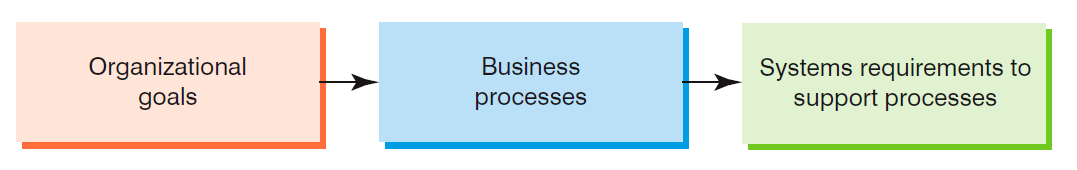
\includegraphics[width=0.8\textwidth]{chapter11/is_plan.png}
					\end{center}
				\end{definition}
			\subsection{Object-Oriented Systems Analysis}
				\begin{definition}{Object-Oriented Systems Analysis}
					Like traditional analysis, problems or potential opportunities are identified.

					With the object-oriented approach, systems analysts are looking for \concept{classes} -- things within the system that have data and action -- rather than entities. These classes are then modelled with the messages and data flow between them.

					\begin{description}
						\item[Object] An instance of a class.
					\end{description}
				\end{definition}
			\subsection{The Systems Analysis Report}
				\begin{definition}{Systems Analysis Report}
					A formal report that concludes system analysis. It should cover:
					\begin{itemize}[nosep]
						\item The strengths and weaknesses of the existing system from a stakeholder's perspective
						\item The user/stakeholder requirements for the new system (also called the \concept{functional requirements})
						\item The organisational requirements for the new system
						\item A description of what the new information system should do to solve a problem
					\end{itemize}
					This report gives managers a good understanding of the problems and strengths of the existing system.
				\end{definition}

		\pagebreak
		\section{Exercises}
			\begin{exercise}{Self-Assessment}
				\begin{enumerate}
					\item \concept{Systems Development} is the activity of creating or modifying existing business systems. It refers to all aspects of the process -- from identifying problems to be solved or opportunities to be exploited, to the implementation and refinement of the chosen solution.
					\item Which of the following people ultimately benefit from a systems development project?
						\begin{enumerate}[label=\alph*., nosep]
							\item computer programmers
							\item systems analysts
							\item[\refstepcounter{enumii}\Circled{\alph{enumii}}] \concept{stakeholders}
							\item senior-level managers
						\end{enumerate}
					\item What factors are essential to the success of certain functional areas of an organisation?
						\begin{enumerate}[label=\alph*., nosep]
							\item[\refstepcounter{enumii}\Circled{\alph{enumii}}] \concept{critical success factors}
							\item systems analysis factors
							\item creative goal factors
							\item systems development factors 
						\end{enumerate}
					\item What employs tools, techniques and methodologies designed to speed application development?
						\begin{enumerate}[label=\alph*., nosep]
							\item[\refstepcounter{enumii}\Circled{\alph{enumii}}] \concept{rapid application development}
							\item joint optimisation
							\item prototyping
							\item extended application development
						\end{enumerate}
					\item Systems performance is usually determined by factors such as fixed investments in hardware and related equipment. True or False? \concept{False}
					\item \concept{Prototyping} takes an iterative approach to the systems development process.
					\item Joint application development involves group meetings in which users, stakeholders, and IS professionals work together to analyse existing systems, propose possible solutions, and define the requirements for a new or modified system. True or false? \concept{True}.
					\item Feasibility analysis is typically done during which systems development stage?
						\begin{enumerate}[label=\alph*., nosep]
							\item[\refstepcounter{enumii}\Circled{\alph{enumii}}] \concept{investigation}
							\item analysis
							\item design
							\item implementation
						\end{enumerate}
					\item Data modelling is most often accomplished through the use of \concept{Entity-relationship Diagrams}, whereas activity modelling is often accomplished through the use of \concept{Data Flow Diagrams}.
					\item The overall purpose of requirements analysis is to determine user, stakeholder, and organisational needs. True or False? \concept{True}.
				\end{enumerate}
			\end{exercise}

	\vbox{\rulechapterend}
\end{document}